\documentclass[12pt, a4paper]{article}%{revtex4-1}
\setlength{\textwidth}{6.9in} \setlength{\textheight}{9.2in}
\hoffset -2.cm \voffset -2.0cm \pagestyle{empty}

\usepackage[utf8]{inputenc}
\usepackage[T1]{fontenc}

\usepackage{xcolor}
\usepackage{pgfplots}
\usepackage{subfigure}
\usepackage{graphicx}


\usepackage{lipsum}
\usepackage{mathtools}
\usepackage{physics}
\usepackage{amsfonts}
\usepackage{amssymb}
\usepackage{amsmath}
\usepackage{amsthm}
\usepackage{import}
\usepackage{tikz}
\usepackage{hyperref} 
\hypersetup{
	pdftex,
	colorlinks=true,
	linkcolor=blue,
	citecolor=red,
	filecolor=magenta,
	urlcolor=blue,
	pdftitle={Article},
	pdfauthor={Author},
}

%\tolerance=1
%\emergencystretch=\maxdimen
%\hyphenpenalty=10000
%\hbadness=10000

%==================================================================================
\begin{document}

\begin{center}
{\Large\bf Investigating an analytic model for neutrino\\ light curves of core-collapse supernovae}

\vspace{5pt}
{\large ASIoP Summer Student Program 2023}

Final Presentation \& Poster Exhibition, Chang-Mao Yang

\vspace{5pt}
\hrule
\vspace{6pt}

\end{center}
	
%_____________________________________________________________________________________
\section{Introduction}

Parameter estimation is crucial in scientific research, especially in data analysis and modeling. Traditional optimization techniques, such as the least square method, often face challenges with increasing parameter dimensionality. The Markov Chain Monte Carlo (MCMC) method, with its Metropolis-Hastings algorithm, emerges as a powerful alternative, finding applications in areas like gravitational wave data analysis.
In this context, coupled oscillators, which offer insights into phenomena like lattice vibrations, become an interesting subject of study. We constructed an experimental system of oscillators connected through springs with unknown constants. Using the MCMC method, we aimed to estimate these unknown spring constants. Our results indicate that MCMC not only enhances computational efficiency but also provides more accurate parameter estimations compared to traditional methods.

%_____________________________________________________________________________________
\section{Experimental Equipment}

Our experimental equipment can be interpreted as shown in FIG. (1), consists of a standard pulley track and two carts. 
	\begin{figure}[h]
	\centering
	\includegraphics[width=0.5\textwidth]{../paper/image/system_cleanup.jpg}
	\caption{Experimental setup of the Coupled Oscillators system.}
	\label{fig:exp-system}
	\end{figure}
These carts are interconnected using three homemade springs made by white iron wire, forming a coupled oscillator system. To capture the oscillators' motion, we employed two ultrasonic distance sensors, housed in 3D-printed frames and connected to an Arduino circuit board. Furthermore, we developed a customized webpage hosted on GitHub for real-time visualization of the displacement data recorded by these sensors. This setup enabled us to measure and document the dynamics of the coupled oscillators effectively.

%_____________________________________________________________________________________
\section{Analytic Model}
Our experimental equipment can be interpreted as shown in following FIG.(2). 
	\begin{figure}[h]\centering
	\import{../paper}{image/figure.tex}
	\caption{Coupled Oscillation system with three springs and two masses.}
	\label{fig:system}
	\end{figure}
The system's Lagrangian is represented by 
\begin{equation}
	L = \frac{1}{2}\sum_{i=1}^{2}m_i \frac{d^2x_i}{dt^2}
		-\frac{k_1x_1^2+k_2\left(x_1-x_2\right)^2+k_3x_2^2}{2},
	\end{equation}
where mi is the mass of ith oscillator and (k1, k2, k3) are the spring constants. Using Euler-Lagrange equation, we obtain a set of the second-order differential equations
	\begin{equation}
	\frac{d^2}{dt^2}\begin{pmatrix}x_1\\ x_2\end{pmatrix} =
	\begin{pmatrix}
	\displaystyle - \frac{k_1+k_2}{m_1}	&\displaystyle  \frac{k_2}{m_1}\\
	\displaystyle  \frac{k_2}{m_2} 		&\displaystyle  -\frac{k_2+k_3}{m_2}
	\end{pmatrix}
	\begin{pmatrix}x_1\\ x_2\end{pmatrix}.
	\end{equation}
After some algebra, the general expressions for the time-dependent displacement x1(t) and x2(t) can be exactly solved.
%_____________________________________________________________________________________
\section{Desired Distribution}
Given the system parameters and initial conditions, the displacements x1(t) and x2(t) of the coupled oscillators can be determined. After measuring the masses and initial positions of the oscillators, the real-time data can be used to estimate the unknown spring constants k1, k2 and k3. The fitting error is defined as:
	\begin{equation}
	\mathrm{err}\left(k_1,k_2,k_3\right) = \sum_{i=1}^{2}\sum_{j=0}^{N-1}\frac{\left(x_i\left(t_j\right) - x_{i,j}\right)^2}{N},
	\end{equation}
where N is the total time steps. The desired distribution for MCMC is
	\begin{equation}
	p\left(k_1,k_2,k_3\right) = \exp\left(-\text{err}\left(k_1,k_2,k_3\right)\right), \quad \text{with }\mathrm{err}\in [0,\infty),
	\end{equation}
Optimized values for k1, k2 and k3 correspond to the distribution's maximum. To enhance optimization accuracy, we applied a Gamma correction to improve the distribution's contrast. The corrected distribution is given by: 
	\begin{equation}
	P = p^{\gamma},\quad p\in (0,1],
	\end{equation}
This Gamma correction ensures a clearer distinction between peak and valley values in the distribution, aiding in the optimization process.

%_____________________________________________________________________________________
\section{Markov Chain Monte Carlo method and Result}
Using the defined distribution function P, we applied the Metropolis-Hastings algorithm within the MCMC method to explore the parameter space of (k1, k2, k3). After sampling 100,000 combinations, we obtained a simulated posterior distribution, visualized using the “Corner.py” package, as shown in FIG. (3.a). 
	\begin{figure}[h]
	\centering
	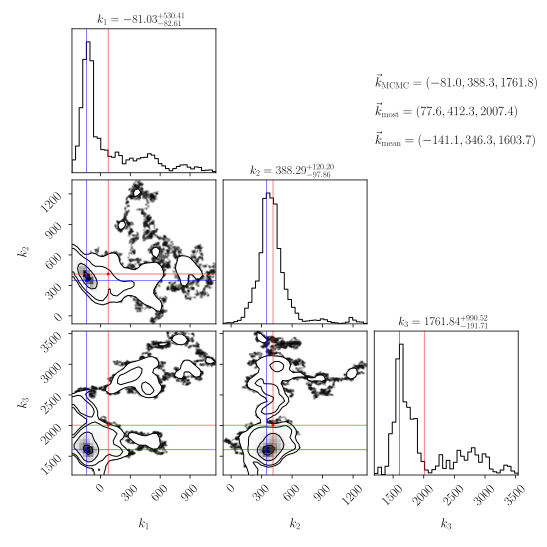
\includegraphics[width=0.5\linewidth]{../paper/image/MCMC_corner.pdf}
	\caption{Posterior distributions of the spring constants $k_1$, $k_2$, and $k_3$ using the corner package. The plots on the main diagonal represent the one-dimensional distributions of each parameter, while the plots in the lower triangle show the two-dimensional distributions between pairs of parameters. The red lines mark the median positions, corresponding to values of $101.03\,(\mathrm{N/m})$, $175.97\,(\mathrm{N/m})$, and $265.02\,(\mathrm{N/m})$ for $k_1$, $k_2$, and $k_3$, respectively, in this figure.}
	\label{fig:MCMC_corner}
	\end{figure}

The main diagonal subplots present the statistical distributions for the spring constants, which, despite some skewness, closely resemble normal distributions. 
FIG. (3.b) compares experimental measurements with numerical calculations based on MCMC-estimated parameters. Despite minor discrepancies, the numerical simulation aligns well with the experimental trends of the coupled oscillators, highlighting the MCMC method's efficiency in parameter estimation for classical physics models.

%_____________________________________________________________________________________
\section{Conclusion}
In this study, we employed the MCMC method, specifically the Metropolis-Hastings algorithm, to analyze the coupled oscillators system. This approach allowed us to navigate the parameter space of the spring constants k1, k2 and k3, resulting in a posterior distribution that mirrors a normal distribution. 
While there were minor variations in the experimental data, the MCMC-derived outcomes closely matched the observed results. Our research underscores the advantage of using the MCMC method for parameter estimation in the context of the coupled oscillators system, as opposed to traditional techniques.
Looking ahead, our focus will be on enhancing the experimental setup and further investigating the system's dynamics by experimenting with springs of different elastic properties. Such efforts aim to deepen our comprehension of coupled oscillators and set the stage for the development of more refined models and analytical methodologies.


%_____________________________________________________________________________________
\section{Reference:}


[1] W.K. Hastings, "Monte Carlo sampling methods using Markov chains and their applications," Biometrika, vol. 57, no. 1, pp. 97–109, 1970.


[2] Zenodo Archive. 2016. “Corner.py: Scatterplot Matrices in Python.” http://dx.doi.org/ 10.5281/zenodo.53155. doi:10.5281/zenodo.53155.
\end{document}






